\documentclass[a4paper,11pt]{report}
\usepackage[T1]{fontenc}
\usepackage[utf8]{inputenc}
\usepackage[polish]{babel}
\usepackage{lmodern}
\usepackage{graphicx}
\usepackage{geometry}

\title{Czas realizacji algorytmów sortowania.
\\Mergesort, Heapsort, Quicksort.}
\author{Monika Litwin 200586}
\begin{document}
\maketitle

\begin{figure}
  \begin{center}
  \textbf{Mergesort}
\\
Algorytmu sortowania Mergesort należy do algorytmów szybkich, czyli posiadających klasę czasowej złożoności obliczeniowej równą \emph{O(nlogn)} lub lepszą. Mergesort w teorii cechuje się właśnie złożonością \emph{O(nlogn)}. Patrząc na wykres można uznać, że tak właśnie zachowuje się zaimplementowane przeze mnie w programie sortowanie merge. 

    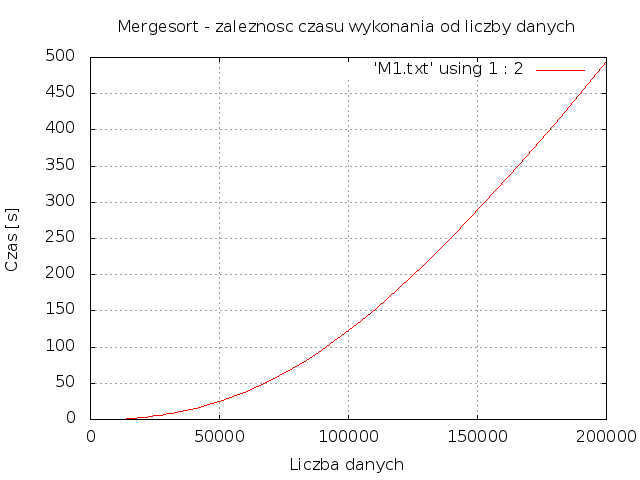
\includegraphics[scale=0.5]{./merge1.png}
    \label{fig:}
  \end{center}
\end{figure}

\begin{figure}
  \begin{center}
  W testach ten typ sortowania wypadł zdecydowanie najgorzej. Okazał się stanowczo najwolniejszy.
    \label{fig:}
  \end{center}
\end{figure}

\begin{figure}
  \begin{center}
  \textbf{Quicksort}
\\Quicksort to prawdopodobnie najczęściej obecnie stosowany algorytm sortowania. Dla średniego przypadku jego złożoność obliczeniowa wynosi \emph{O(nlogn)}. Zbliżoną do niej złożoność obliczeniową uzyskano w testach, zobrazowanych poniższym wykresem.
\\
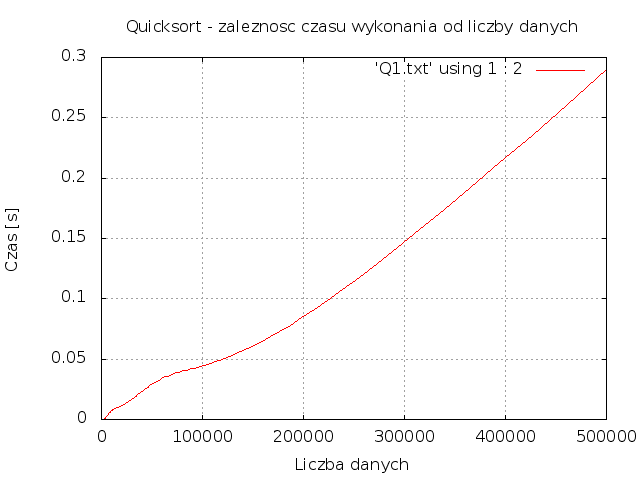
\includegraphics[scale=0.5]{./quick1.png}
  \end{center}
\end{figure}

\begin{figure}
  \begin{center}

Algorytm ten posiada przypadek optymistyczny i pesymistyczny, których złożoność obliczeniowa znacznie się różni. Przypadek pesymistyczny to taki, kiedy sortujemy uporządkowaną już tablicę. Wówczas podtablica nie jest praktycznie dzielona, ale odpada od niej jedynie element osiowy, a pozostałą część podtablicy należy dzielić dalej.Prawdopodobnie właśnie taki przypadek otrzymaliśmy, gdy zadane było 10 powtórzeń algorytmu. Tylko za pierwszym razem wektor faktycznie sortowano, pozostałe 9 razy sortowany był, już wcześniej uporządkowany wektor. Obraz tego mamy na wykresie poniżej.
\\
    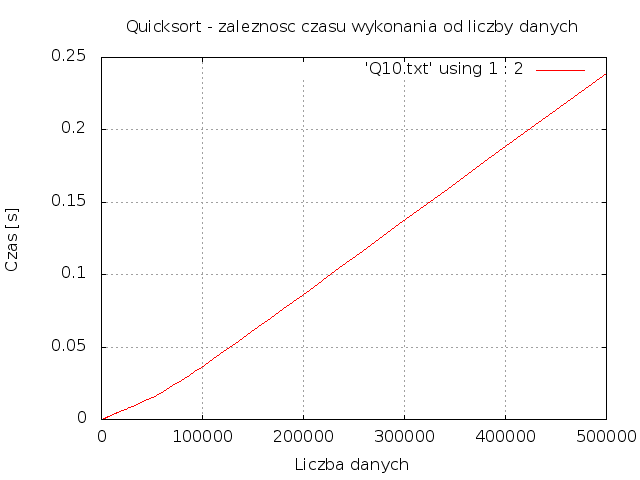
\includegraphics[scale=0.5]{./quick10.png}
    \label{fig:}
  \end{center}
\end{figure}

\begin{figure}
  \begin{center}
W odróżnieniu od algorytmu sortowania megre, tutaj przy podziale danych na podtablice, dąży się do tego, aby podział na podtablice był jak najbardziej równomierny(co powoduje znaczne zwiększenie złożoności w przypadku niekorzystnym). W sortowaniu merge, podział tablicy jest maksymalnie uproszczony - zawsze jest dzielona na połowy, bez wnikania w ułożnie danych, Faktyczne sortowanie ma miejsce w trakcie scalania tablic. W Quicksort jest odwrotnie - sortowanie ma miejsce w trakcie podziału, a łączenie jest automatyczne.
    \label{fig:}
  \end{center}
\end{figure}

\begin{figure}
  \begin{center}
  \textbf{Heapsort}
  \\Sortowanie typu heap również zalicza się do algorytmów szybkich. Cechuje się złożonością liniowo logarytmiczną. Jest nieco wolniejszy niż quick, ale w odróżnieniu od tego, wykazuje bardzo małą wrażliwość na postać danych i utrzymuje stałą złożoność czasową. 
  \\
    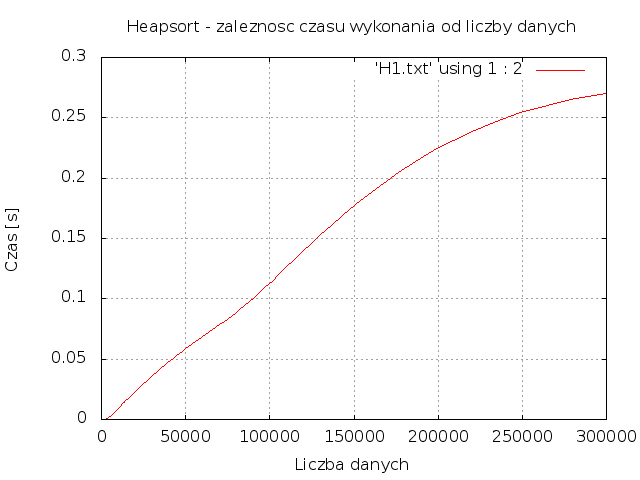
\includegraphics[scale=0.5]{./heap1.png}
    \label{fig:}
  \end{center}
\end{figure}

\end{document}
